\subsection{ScaFi}

\textbf{\ac{ScaFi}}\footnote{\url{https://github.com/scafi}} is an
open-source aggregate computing framework for the Scala programming language,
providing a usable internal \ac{DSL} for aggregate specifications and a
platform for the simulation and execution of such specifications
\cite{ScaFi-Documentation}.

In \ac{ScaFi}, the core concepts of field calculus are modelled by a
\textbf{trait} (i.e. an interface) like the one reported in Listing
\ref{listing:scafi-field-calculus} \cite{FieldCalculus-AggregateComputing},
whose methods represent the constructs of field calculus.

\begin{lstlisting}[
  language=Scala,
  caption={The core constructs of field calculus, represented as a trait,
  abstracting over the actual organization within ScaFi.},
  captionpos=b,
  label={listing:scafi-field-calculus}
]
trait FieldCalculus:
  def nbr[E](exp: => E): E
  def rep[E](exp: => E)(evolve: E => E): E
  def foldhood[E](exp: => E)(accumulate: (E, E) => E)(nbrExp: => E): E
  def aggregate[E](exp: => E): E

  // platform interactions
  def mid: Id
  def sense[V](name: String): V
  def nbrvar[V](name: String): V
\end{lstlisting}


\ac{ScaFi} provides no explicit reification for computational fields. Indeed,
any Scala expression is treated implicitly as a field calculus expression,
yielding a computational field. For instance, the expression "$1+2$" yields
constant uniform computational field holding the value $3$ at any point in
space and time, obtained as the point-wise summation of a field of "$1$"s and a
field of "$2$"s (Figure \ref{figure:constant-uniform-field}).

\begin{figure}[h]
  \centering
  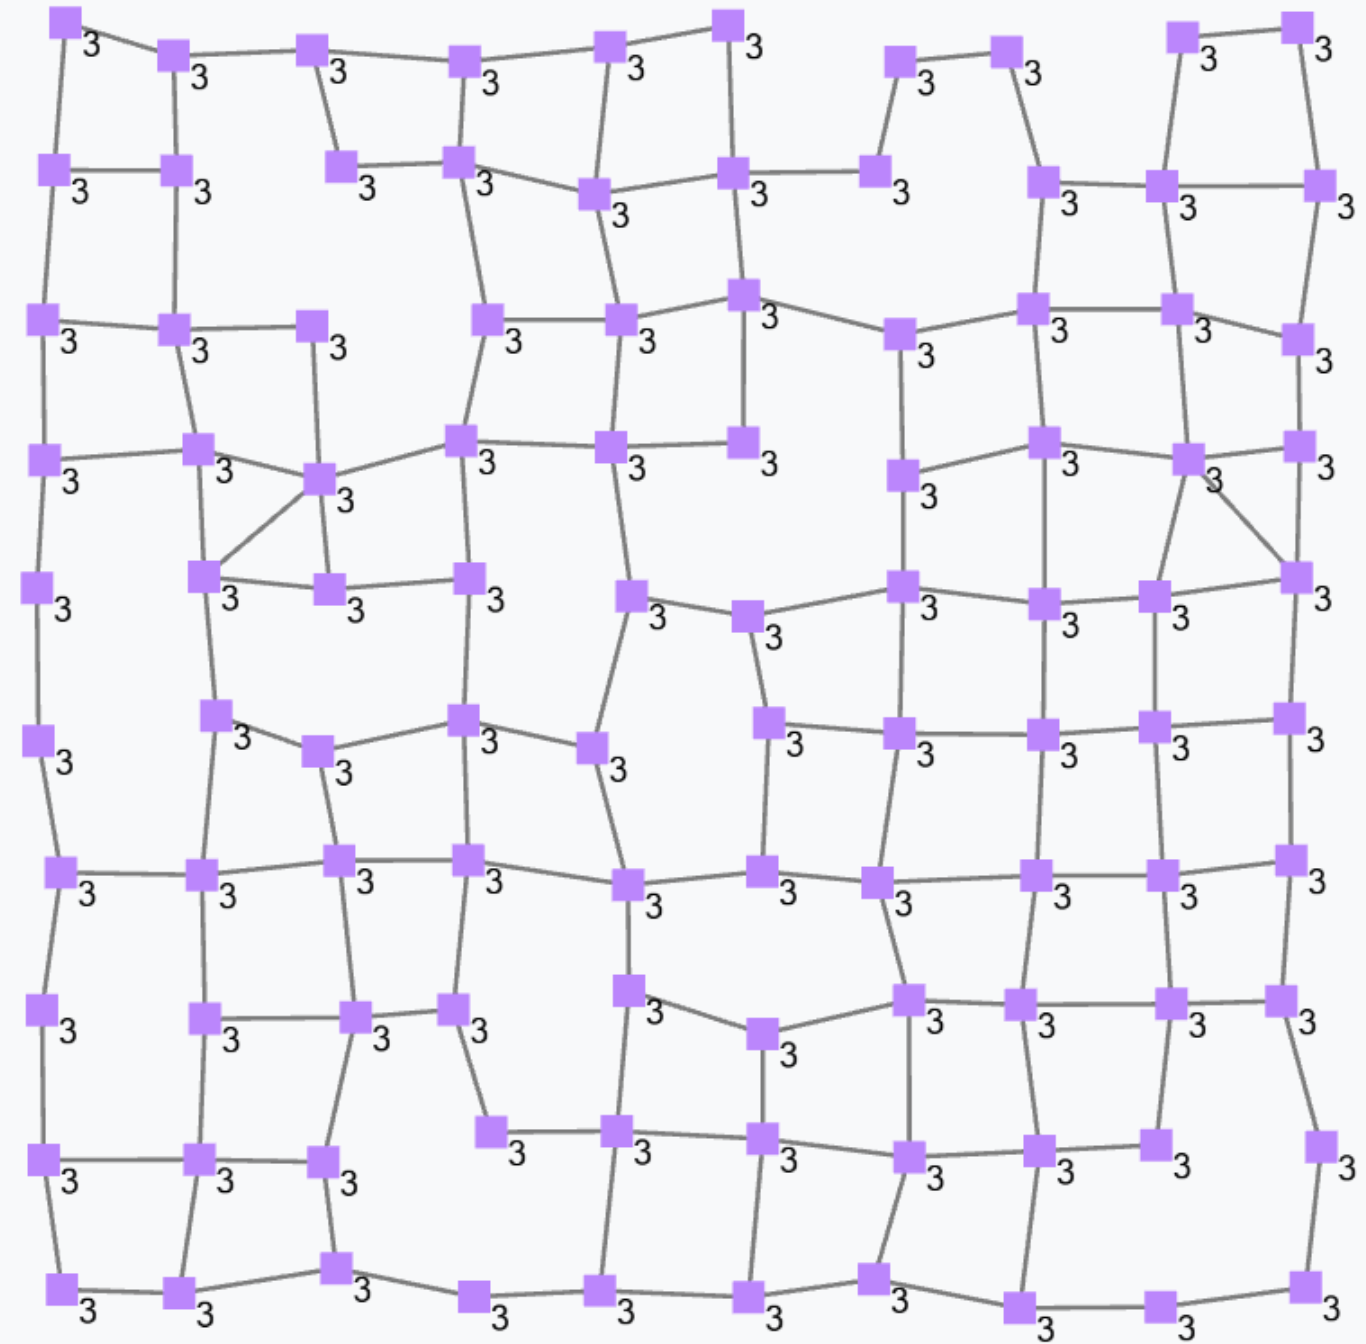
\includegraphics[width=0.60\textwidth]{resources/figures/constant-uniform-field.png}
  \caption{
    A graph representing an aggregate of devices (\textit{nodes}) and their
    neighboring relations (\textit{edges}). In particular, it represents the
    computational field yielded by the expression "$1+2$"
    \cite{ScaFi-Documentation}.
  }
  \label{figure:constant-uniform-field}
\end{figure}

Despite being equivalent, the semantics of \ac{ScaFi} differ from the semantics
of field calculus for some operators: evolution over space is implemented with
a combination of the \texttt{nbr} and \texttt{foldhood} operators, the latter
exploiting the former to accumulate the values of neighbors in each device
(i.e. \texttt{nbr} does not yield a neighboring value directly as in field
calculus); restriction is implemented using the \texttt{aggregate} operators,
which handles selective partitioning; evolution over time with \texttt{rep}
follows the same semantics as field calculus.

Additionally, \ac{ScaFi} provides contextual operators that handle interactions
with the underlying platform, namely \texttt{mid}, which computes the field of
the device identifiers in the aggregate, \texttt{sense}, which computes a field
of the values perceived by a specific sensor from the environment (e.g. a field
of temperatures), and \texttt{nbrvar}, which computes a field mapping each
neighbor to a value perceived by a specific sensor from the environment (e.g. a
field of distances with each neighbor).

The core \ac{DSL} can be extended with \textbf{mixins} to provide higher-level
primitives and operators. \ac{ScaFi} already includes some built-in extensions,
such as the resilient aggregate computing blocks (Listing
\ref{listing:scafi-aggregate-computing}).

\begin{lstlisting}[
  language=Scala,
  caption={The core constructs of aggregate computing, represented as a mixin
  for field calculus, abstracting the actual organization within ScaFi.},
  captionpos=b,
  label={listing:scafi-aggregate-computing}
]
trait AggregateComputing:
  self: FieldCalculus =>
  // aggregate computing blocks
  def G[V](source: Boolean, initial: V, accum: V => V, metric: () => Double): V
  def C[P: Bounded, V](potential: P, accum: (V, V) => V, local: V, nullV: V): V
  def T[V: Numeric](initial: V, floor: V, decay: V => V): V
  def S(grain: Double, metric: () => Double): Boolean

  // derived operators
  def branch[E](cond: => E)(th: => E)(el: => E): E
  def mux[E](cond: => E)(th: => E)(el: => E): E
  def share[E](exp: => E)(evolve: (E, () => E) => E): E
\end{lstlisting}



The higher-level primitives in \ac{ScaFi} include but are not limited to the
already presented \texttt{G}, \texttt{C} and \texttt{T} blocks of aggregate
computing, an additional \texttt{S} block, which handles sparse leader election
based on proximity, a \texttt{branch} operator, implementing the branching
expression of field calculus (relying on
\texttt{aggregate})\footnote{conditional computation without partitioning is
implemented by the \texttt{mux} operator instead, which is equivalent to an
\textit{if-then-else} expression in Scala.}, and a new \texttt{share} operator,
which handles the evolution over time of a neighboring value (indeed a
combination of the behaviors of \texttt{rep} and \texttt{nbr} in field
calculus, albeit much more efficient \cite{ScaFi-ShareOperator}).

The execution of a \ac{ScaFi} specification is performed by the underlying
platform, which adopts an \textit{asynchronous} \textbf{round-based} execution
model, in which a round is the computation required for an individual device to
produce its next output based on the aggregate specification. A round consists
of the following three steps in order:
\begin{enumerate}
  \item \textbf{sense}: the device updates its current \textbf{context} (i.e.
        all known information in its perspective), by retrieving its previous
        output, the information perceived through its \textit{sensors} from the
        local environment and the messages arriving from neighboring devices;
  \item \textbf{compute}: the device computes its current output by executing
        the aggregate specification against its current context. The output of
        a device is an abstract syntax tree, tracking the structure of the
        executed aggregate specification for alignment. In particular, the root
        of the tree contains the final result of the computation, while the
        roots of its sub-trees contain the results of sub-computations.
  \item \textbf{interact}: the device broadcasts some information extracted
        from its output (called an \textbf{export}) to neighboring devices and
        updates the local environment through its \textit{actuators}. The
        export can be derived from the output of the device by searching in the
        abstract syntax tree for operations involving communication (e.g.
        sub-trees depending on \textbf{nbr}).
\end{enumerate}

Support for simulation is also implemented by several \ac{ScaFi} modules or
through integration with third-party simulators (e.g.
Alchemist\footnote{\url{https://github.com/AlchemistSimulator/Alchemist}}
\cite{Alchemist}).
